\documentclass[12pt]{article} % use larger type; default would be 10pt

%packages
\usepackage[utf8]{inputenc} % set input encoding (not needed with XeLaTeX)
\usepackage{fancyhdr}
\usepackage{float}
\usepackage{geometry}
\usepackage{ulem}
\usepackage{soul}
\usepackage{color}
\usepackage{graphicx}
\usepackage{hyperref}
\usepackage{array}
\usepackage{caption}
\usepackage{titling}
\usepackage{enumerate} 
\usepackage[dvipsnames]{xcolor}
\usepackage{amsmath}
\usepackage{amssymb}
\usepackage[compact]{titlesec}


 %put box around figure captions
\makeatletter
\long\def\@makecaption#1#2{%
  \vskip\abovecaptionskip
  \sbox\@tempboxa{\fbox{#1: #2}}%
  \ifdim \wd\@tempboxa >\hsize
    \fbox{\parbox{\dimexpr\linewidth-2\fboxsep-2\fboxrule}{#1: #2}}\par
  \else
    \global \@minipagefalse
    \hb@xt@\hsize{\hfil\box\@tempboxa\hfil}%
  \fi
  \vskip\belowcaptionskip}
\makeatother

%reduce space between 
\titlespacing{\section}{0pt}{*1}{*0}
\titlespacing{\subsection}{0pt}{*1}{*0}
\titlespacing{\subsubsection}{0pt}{*0}{*0}


%no indent and modify distance between paragraphs
\setlength\parindent{0pt}
\setlength\parskip{12pt}

%set margins and line spacing
\geometry{margin=1in}
\linespread{1.2}
\geometry{letterpaper}

%math operators
\DeclareMathOperator{\E}{\mathbb{E}}

%set up header and page numbering
\pagestyle{fancy}
\lhead{CS 155 Set 6}
\rhead{Timothy Liu}
\pagenumbering{arabic}



\title{CS155 Set 6}
\author{Timothy Liu}

\begin{document}


\maketitle

\newpage

\section{Problem 1}
\subsection{Problem A}
\subsubsection{Part i}

$$p(x|y = c) = p\bigg((x_1|y=c), (x_2|y=c), (x_3|y = c).....(x_j|y=c)\bigg)$$
$$p(x|y = c) = \prod_{j=1}^D \theta_{xjc}$$

This requires $O(DC)$ parameters to be stored.

\subsubsection{Part ii}
We would need to store $O(D 2^D C)$ parameters because we have to store one parameter for every combination of other parameters and then multiply this by the number of values of C. This is drastically more parameters to store.

\subsection{Problem B}
The Naive Bayes model has fewer parameters, and for a small training set it will be less prone to overfitting. The Naive Bayes will have lower test set error.

\subsection{Problem C}
If the sample size N is very large, then the full model will have lower test set error. The larger number of parameters will be able to better capture the large sample size, and it will not have the same overfitting problem if the training set is large enough.

\subsection{Problem D}
Making a prediction with Naive Bayes requires multiplying D parameters together and there are C classes, making this a $O(DC)$ operation.  In the complete case, we must multiply D parameters together, making it a $O(D)$ operation.

\section{Problem 2}

\subsection{Problem A}
\begin{figure}[H]
	\makebox[\textwidth][c]{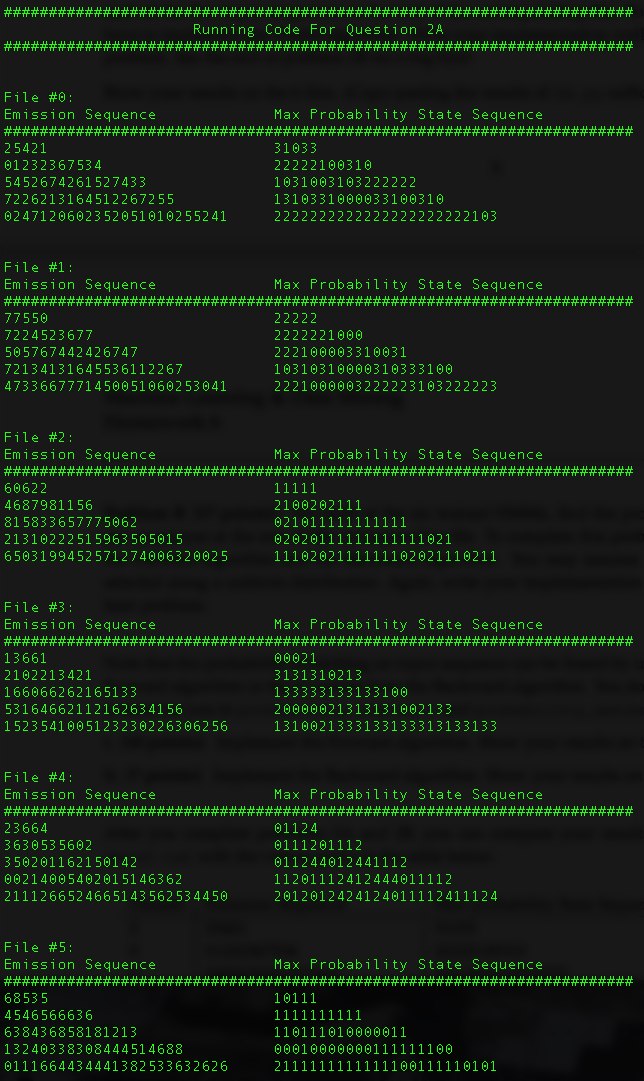
\includegraphics[width=4.5in]{2A.png}}
	\vspace{-10mm}
	\caption{Output for viterbi algorithm.}
\end{figure}

\subsection{Problem B}
\subsubsection{Part i}
\begin{figure}[H]
	\makebox[\textwidth][c]{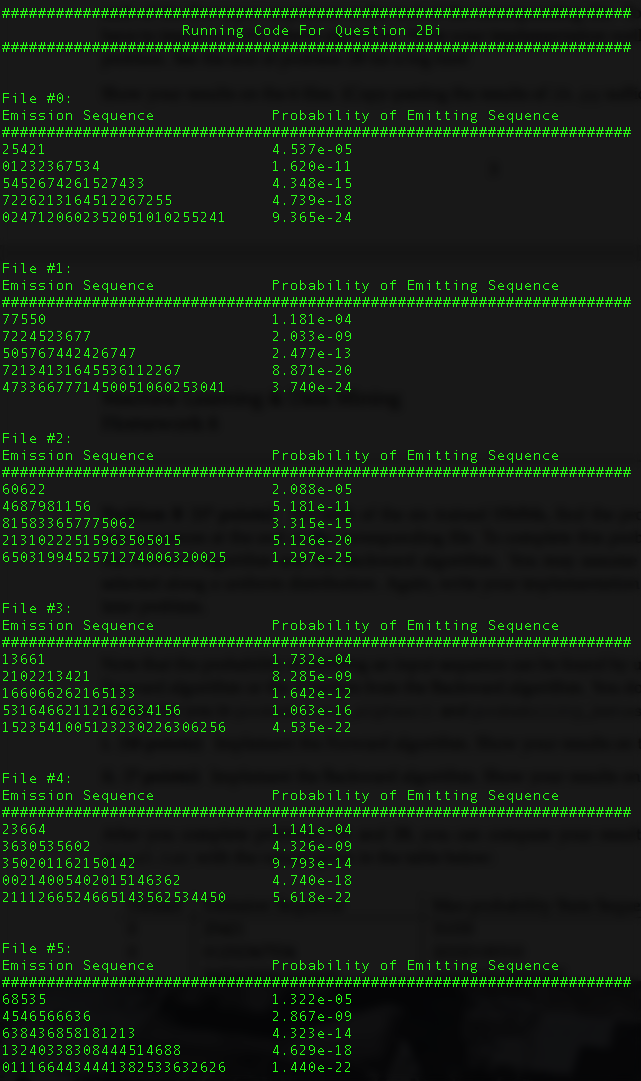
\includegraphics[width=4.5in]{2Bi.png}}
	\vspace{-10mm}
	\caption{Probabilities calculated from forwards algorithm.}
\end{figure}

\subsubsection{Part ii}

\begin{figure}[H]
	\makebox[\textwidth][c]{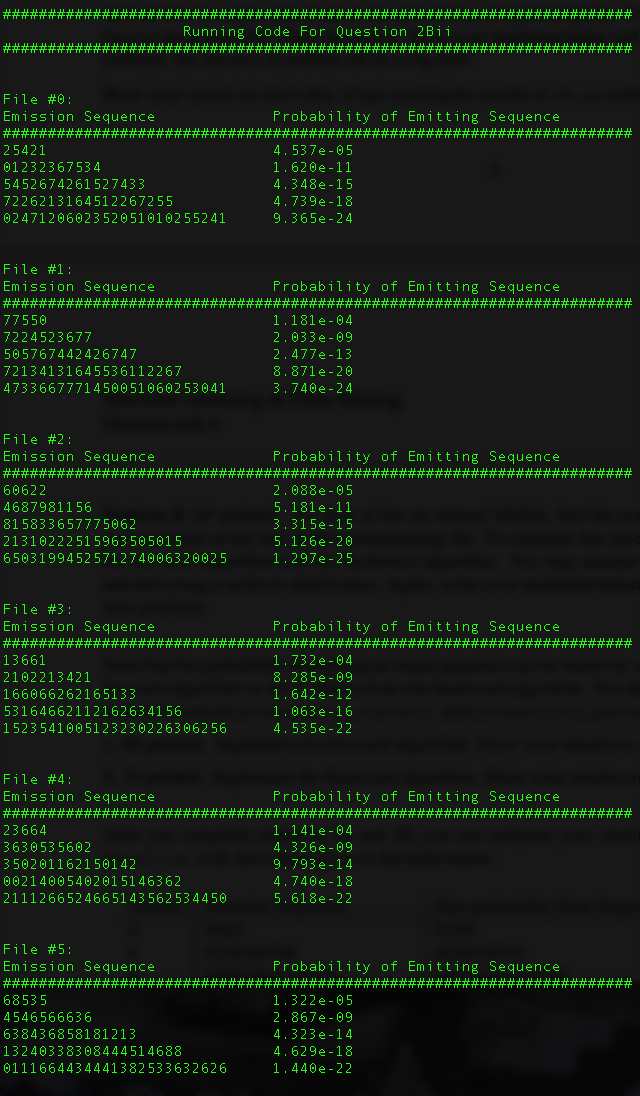
\includegraphics[width=4.5in]{2Bii.png}}
	\vspace{-10mm}
	\caption{Probabilities calculated from backwards algorithm.}
\end{figure}

\subsection{Problem C}
Transition matrix:
\begin{figure}[H]
	\makebox[\textwidth][c]{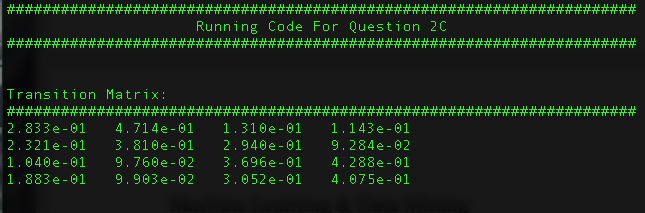
\includegraphics[width=7in]{2CT.png}}
	\vspace{-10mm}
	\caption{Transition matrix.}
\end{figure}

Observation matrix:
\begin{figure}[H]
	\makebox[\textwidth][c]{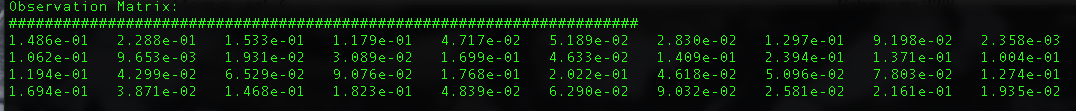
\includegraphics[width=7in]{2CO.png}}
	\vspace{-10mm}
	\caption{Observation matrix.}
\end{figure}

\newpage
\subsection{Problem D}

Transition matrix:
\begin{figure}[H]
	\makebox[\textwidth][c]{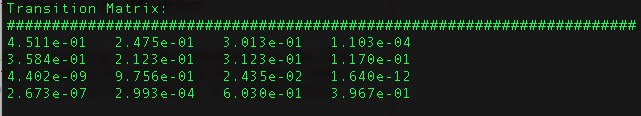
\includegraphics[width=7in]{2DT.png}}
	\caption{Learned transition matrix from unsupervised learning.}
\end{figure}

Observation matrix:
\begin{figure}[H]
	\makebox[\textwidth][c]{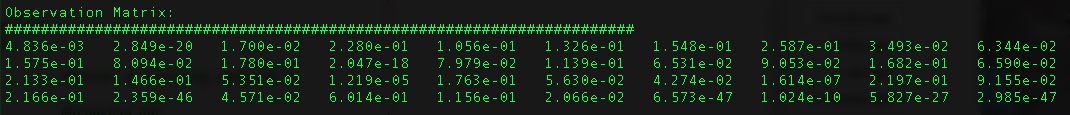
\includegraphics[width=7in]{2DO.png}}
	\caption{Learned observation matrix from unsupervised learning.}
\end{figure}

\subsection{Problem E}
The supervised model is likely more accurate because it's trained on both the values and the labels. The supervised model is guaranteed to have the correct states while the unsupervised model is guessing at how many states there are. The unsupervised transition matrix sometimes pushes the transition probability between two states to near zero, which the supervised matrix does not. The two transition matrices have little resemblance. Similarly, the observation matrix for unsupervised has some values very close to zero, which the transition matrix does not. The supervised matrix is likely a better representation because it's trained on labeled data. One way to improve the unsupervised model is to either feed it even more data or to somehow include regularization.

\subsection{Problem F}

\begin{figure}[H]
	\makebox[\textwidth][c]{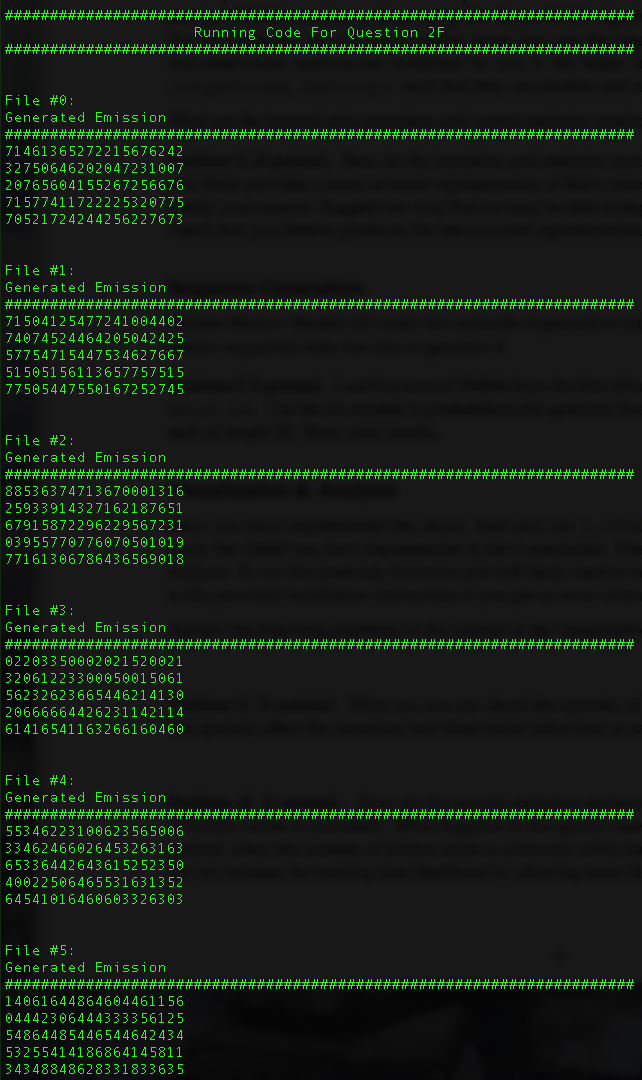
\includegraphics[width=4.5in]{2F.png}}
	\vspace{-10mm}
	\caption{Emitted sequences.}
\end{figure}

\subsection{Problem G}
Word cloud visualization of constitution:

\begin{figure}[H]
	\makebox[\textwidth][c]{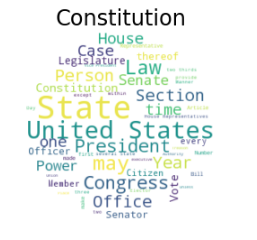
\includegraphics[width=4.5in]{2Hw.png}}
	\vspace{-10mm}
	\caption{Word cloud representing US constitution.}
\end{figure}

\begin{figure}[H]
	\makebox[\textwidth][c]{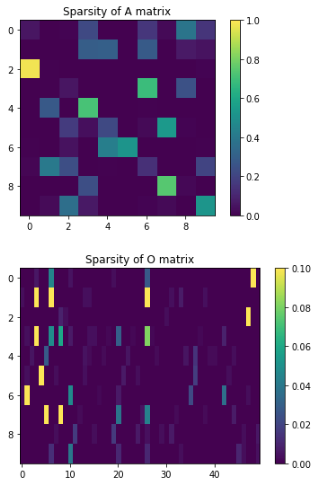
\includegraphics[width=4.5in]{2G.png}}
	\vspace{-10mm}
	\caption{Sparsity of matrices.}
\end{figure}

Both the trained A and O matrices are fairly sparse. A large portion of both matrices are 0. This means that there are many possible state transitions that never happen, or there are some states that cannot emit certain observations. This makes sense, as there are some states - such as verb to verb - that may be unlikely.

\subsection{Problem H}

\begin{figure}[H]
	\makebox[\textwidth][c]{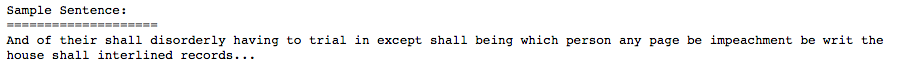
\includegraphics[width=7in]{gen1_state.png}}
	\caption{Emission with 1 state.}
\end{figure}

\begin{figure}[H]
	\makebox[\textwidth][c]{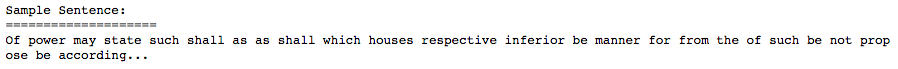
\includegraphics[width=7in]{gen2_state.png}}
	\caption{Emission with 2 states.}
\end{figure}

\begin{figure}[H]
	\makebox[\textwidth][c]{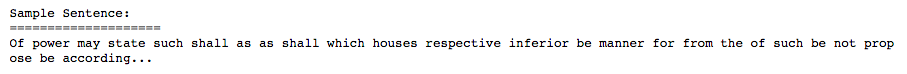
\includegraphics[width=7in]{gen4_state.png}}
	\caption{Emission with 4 states.}
\end{figure}

\begin{figure}[H]
	\makebox[\textwidth][c]{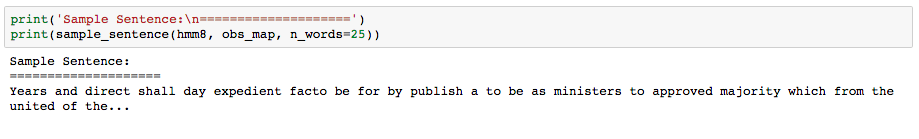
\includegraphics[width=7in]{gen10_state.png}}
	\caption{Emission with 10 states.}
\end{figure}

\begin{figure}[H]
	\makebox[\textwidth][c]{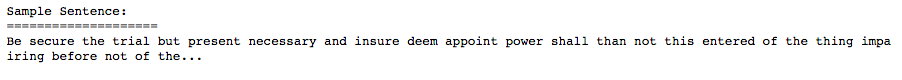
\includegraphics[width=7in]{gen16_state.png}}
	\caption{Emission with 16 states.}
\end{figure}

The sample emissions become somewhat more meaningful as the number of states changes. In the special case of only one state, the sentence makes no grammatical sense. Adding more hidden states will likely improve performance but only to a certain point. If there are too many hidden states, then the HMM may try to extract meaning that does not exist.

\subsection{Problem I}

State 4 seems to represent descriptors of the legislative branch. The words ``congress," ``house," and ``senate" all appear in the word cloud. This states differs from some others like state 8, which has no dominant words. The words in state 4 all appear to be describing something similar, rather than being a part of speech.


\end{document}
